\chapter{Reservation system Shongo}
In this chapter, we will introduce the reservation system Shongo for which this thesis will make \hyperref[rest]{REST API} extension.

Currently, at version v0.9.3, Shongo is a generic system used for managing resources.
Its primary function is to manage resources reservations for virtual meetings and any physical resources, such as physical meeting rooms, vehicles or parking places.
It allows administrators to define available resources (e.g., H.323 MCU or Adobe
Connect Server) and users to reserve the resources mentioned before. \cite{shongo}

CESNET association develops the system as an open-source project available at \href{https://github.com/shongo/shongo}{Github repository}, and it is currently deployed in these domains:
\begin{itemize}
    \item \url{https://meetings.cesnet.cz} - reservation system for H.323/SIP and Adobe Connect virtual rooms within CESNET videoconferencing infrastructure
    \item \url{https://meetings.cesnet.cz/ceitec} - reservation system for physical rooms of CEITEC - Central European Institute of Technology
    \item \url{https://meetings.cesnet.cz/cuni/} - reservation system for users led in authentication system of Charles University \footnote{\url{https://cuni.cz/}}.
\end{itemize}

Users can log in using their profile from any organization belonging to the Czech academic identity federation \footfullcite{eduid}.
After logging in, they can freely use the system and request reservations for available resources.

\enquote{CESNET is an association of universities and the Academy of Sciences of the Czech Republic that operates and develops a national e-infrastructure for science, research and education, including a computer network, computing grids, data repositories, collaborative environments and offering a wide range of services.} \cite{cesnet}

\section{Architecture}
% This section is mostly referenced from another thesis \footfullcite{pavelka2016shongo}, my primary learning material for how the Shongo system works.
I have drawn information for this section from shongo api documentation \footfullcite{shongoapi} and another thesis \footfullcite{pavelka2016shongo}.

The system is composed of a few separate modules. Their interconnections are shown in \Cref{architecture}.
\begin{figure}[!ht]
  \centering
  \caption{Shongo architecture}
%   % generated by Plantuml 1.2018.13      
\definecolor{plantucolor0000}{RGB}{168,0,54}
\definecolor{plantucolor0001}{RGB}{254,254,206}
\definecolor{plantucolor0002}{RGB}{0,0,0}
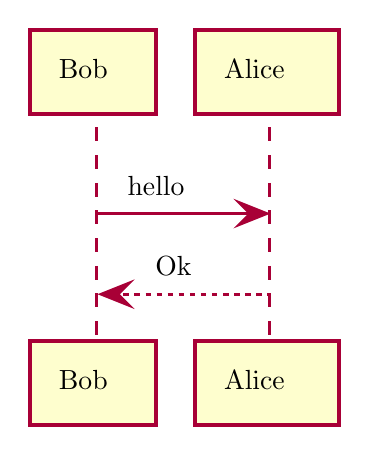
\begin{tikzpicture}[yscale=-1
,pstyle0/.style={color=plantucolor0000,line width=1.0pt,dash pattern=on 5.0pt off 5.0pt}
,pstyle1/.style={color=plantucolor0000,fill=plantucolor0001,line width=1.5pt}
,pstyle2/.style={color=plantucolor0000,fill=plantucolor0000,line width=1.0pt}
]
\draw[pstyle0] (32pt,38.2969pt) -- (32pt,116.5625pt);
\draw[pstyle0] (94.6593pt,38.2969pt) -- (94.6593pt,116.5625pt);
\draw[pstyle1] (8pt,3pt) rectangle (53.6593pt,33.2969pt);
\node at (15pt,10pt)[below right,color=black]{Bob};
\draw[pstyle1] (8pt,115.5625pt) rectangle (53.6593pt,145.8594pt);
\node at (15pt,122.5625pt)[below right,color=black]{Bob};
\draw[pstyle1] (67.6593pt,3pt) rectangle (119.6357pt,33.2969pt);
\node at (74.6593pt,10pt)[below right,color=black]{Alice};
\draw[pstyle1] (67.6593pt,115.5625pt) rectangle (119.6357pt,145.8594pt);
\node at (74.6593pt,122.5625pt)[below right,color=black]{Alice};
\draw[pstyle2] (83.6475pt,65.4297pt) -- (93.6475pt,69.4297pt) -- (83.6475pt,73.4297pt) -- (87.6475pt,69.4297pt) -- cycle;
\draw[color=plantucolor0000,line width=1.0pt] (32.8296pt,69.4297pt) -- (89.6475pt,69.4297pt);
\node at (39.8296pt,52.2969pt)[below right,color=black]{hello};
\draw[pstyle2] (43.8296pt,94.5625pt) -- (33.8296pt,98.5625pt) -- (43.8296pt,102.5625pt) -- (39.8296pt,98.5625pt) -- cycle;
\draw[color=plantucolor0000,line width=1.0pt,dash pattern=on 2.0pt off 2.0pt] (37.8296pt,98.5625pt) -- (94.6475pt,98.5625pt);
\node at (49.8296pt,81.4297pt)[below right,color=black]{Ok};
\end{tikzpicture}

%   \includegraphics{assets/architecture}
  \makebox[\textwidth]{\includegraphics[width=\paperwidth]{assets/architecture}}
  \label{architecture}
\end{figure}

\subsection{Controller} \label{controller}
The controller module is the heart of the Shongo system. Its primary role is to plan requested reservations (\emph{Scheduler} sub-component) and assign necessary resources to them. Its secondary roles are informing users about their reservations (\emph{NotificationManager} sub-component) and administrate remote virtual resources (\emph{Executor} sub-component) via connected \hyperref[connector]{connectors}. Furthermore, last but not least, save this information to the relational database \emph{PostgreSQL}.

These functionalities are made available for other components with the \emph{Application programming interface} (API) via protocol \emph{XML-RPC}.

\subsection{Connector} \label{connector}
Connector is component that enable users to connect to video rooms with their devices (PC, tablet, smartphone, ...).

It is responsible for establishing, maintaining and monitoring connections with remote virtual resources.
It contains implementations for \emph{Device Agent}s where each \emph{Device Agent} can mediate a specific device (e.g. Adobe Connect, Pexip) functions to the controller using the device's API.
The controller communicates with the connector using the JADE (Java Agent DEvelopment) framework, which enables the connection of multiple connectors to a single controller.

\subsection{Authentication server}
The authentication server authenticates incoming requests for the controller component, authenticates users, finds users from various identity providers and gets information about users for the web client.
Besides that, it also manages the authentication layer of the web conference system Adobe Connect. This layer uses the user's information gained after logging in via system Shibboleth \footnote{Shibboleth, \url{https://www.shibboleth.net/}}.

\subsection{Web client} \label{webclient}
The web client is the system's primary interface for users. Using frameworks \emph{SpringMVC} and \emph{AngularJS}, it generates web pages with data gained from the controller's services.

Thanks to this component, users can authenticate via OpenID Connect \footnote{OpenID Connect, \url{https://openid.net/connect/}} and request a reservation for any available resource comfortably via the web.

\subsection{Command line client}
The command line client is the controller's additional interface used for administration. It enables system administrators to manage resources, user, groups and reservation requests which is not possible using the web client.
